%!TEX root = ../../thesis.tex

\section{Application to {CARMENES} spectra}

One of the main reasons for focusing on the extending the work of\citet{figueira_radial_2016} was to analyse the differences in {RV} precision of synthetic spectra and the observed \nir{}.
This is important for the community to understand the accuracy of synthetic spectra.
\citet{artigau_optical_2018} recently found band-specific discrepancies in the theoretical precision between real and synthetic \nir{} spectra of Barnard's Star.
In 2018 {CARMENES} openly released a spectral library containing one spectrum for each target in their 324 M-dwarf {RV} survey \citet{reiners_carmenes_2018}.
With this they provide details on the empirical \(\delta V_{rms}\) measured during their {RV} processing with their {RV} analysis code, {SERVAL} \citep{zechmeister_spectrum_2018}, using all available spectra of each target.
Spectra from this library will be used to compare the theoretical precision of observed {CARMENES} spectra to synthetic models.
This work is still in the preliminary stages but the progress so far will be demonstrated here.

\subsection{Target selection}
\label{subsec:carmense_targets}
To analysis the precision in different spectral types a few specific M-dwarfs were selected.
The 324 spectra of the {CARMENES} M-dwarf library from \citet{reiners_carmenes_2018} are available at \href{http://carmenes.cab.inta-csic.es/gto/}{http://carmenes.cab.inta-csic.es/gto/}, along with the achieved \snr{} in the visible and \nir{} spectra.

The spectral library was downloaded and divided into spectral type and ordered by the {SNR} achieved in the \nir{}, to select targets at the high \snr{} end.
To cover the M-dwarf range targets were selected near each of the spectral types M0, M3, M6 and M9.
For each spectral type (within $\pm0.5$) two stars are selected that have high {SNR} values.
One of the two selected targets for the M3 type is Barnard's star which has been analysed extensively in~\citet{artigau_optical_2018}, in particular with CRIRES spectra for the \nir{} domain, allowing for direct comparisons between the two works.
The other criteria was to try select targets with a varied range of \Logg and \feh{} values if possible.

The selected targets from the {CARMENES} library are provided in \cref{tab:carmenes_selection_updated}.
The spectral parameters (\Teff{}, \Logg{}, \feh{}) for these targets are from \citep{passegger_carmenes_2018, rajpurohit_exploring_2018} who performed spectral fitted of the {CARMENES} spectra with the {PHOENIX-ACES} and {BT-Settl} models respectively.
The uncertainties in the \citet{rajpurohit_exploring_2018} parameters are \(\sigma_{\teff{}}\)=100\K{}, \(\sigma_{\logg{}}\)=0.3, and \(\sigma_{\feh{}}\)=0.3 while the uncertainties on the 
\citep{passegger_carmenes_2018} values are \(\sigma_{\teff{}}\)=51\K{}, \(\sigma_{\logg{}}\)=0.07, and \(\sigma_{\feh{}}\)=0.16.
There are gaps in the \citet{passegger_carmenes_2018} values for stars that have the lower \snr{} levels as they are more difficult to analyse/fit.
Neither one has parameters for Luyten's Star, for which the parameters given are from {SIMBAD}.

\begin{landscape}
    %!TEX root = ../../thesis.tex

\begin{table}[h]
    \centering
    \begin{threeparttable}
        \caption[{CARMENES} targets for {RV} precision analysis.]{Selected {CARMENES} targets with stellar parameters from both~\citet{rajpurohit_exploring_2018} and~\citet{passegger_carmenes_2018}.}
        \begin{tabular}{lllcccccccc}
            %\small
            \toprule
            & & & & & \multicolumn{3}{c}{\citet{rajpurohit_exploring_2018}} & \multicolumn{3}{c}{\citet{passegger_carmenes_2018}} \\
            Karmn & Name & SpT & V & \(\snr{}_{\nir{}}\) & \Teff{} & \Logg{} & \feh{} & \Teff{} & \Logg{} & \feh{} \\
            &  &  & mag &  & \K{} & \si{\centi\metre\per\second\squared} & & \K{} & \si{\centi\metre\per\second\squared} &  \\
            \midrule
            J20533+621 & BD+61 2068     & M0.5 & 8.6  & 257 & 3900          & 5.5 & -0.5           & 3828 & 4.71 & 0.03 \\
            J04290+219 & BD+21 652      & M0.5 & 8.3  & 212 & 4000          & 5.5 & 0.5            & 4194 & 4.59 & 0.20 \\
            J07274+052 & Luyten's Star  & M3.5 & 9.9  & 254 & 3467\tnote{a} & -   & -0.1\tnote{a}  & -    & -    & -    \\
            J17578+046 & Barnard's Star & M3.5 & 9.5  & 236 & 3400          & 5.5 & 0.1            & 3278 & 5.10 & -0.12 \\
            J11055+435 & WX UMa         & M5.5 & 14.5 & 140 & 3000          & 5.5 & 0.3 & - & - & - \\
            J10564+070 & CN Leo         & M6.0 & 13.5 & 133 & 2900          & 5.4 & 0.1 & - & - & - \\
            J18356+329 & LSR J1835+3259 & M8.5 & 18.3 & 50  & 2400          & 5.0 &-0.1 & - & - & - \\
            J04198+425 & LSR J0419+4233 & M8.5 & 11.1 & 42  & 2400          & 4.9 & 0.1 & - & - & - \\
        \bottomrule
        \end{tabular}\label{tab:carmenes_selection_updated}
        \begin{tablenotes}
            \item [a] {From SIMBAD.}
        \end{tablenotes}
    \end{threeparttable}
\end{table}

\end{landscape}



\textbf{BELOW HERE IS Unfinished}


\subsection{Preparation of {CARMENES} spectra}
This work in telluric correcting all spectra chosen has been hampered by the difficulty faced in correcting the {CARMENES} spectra from telluric lines.
There have been issues achieving a reliable telluric correction with the Molecfit software on the {CARMENES} spectra (private-communication Ulmer-mol (2018)).
At this stage only one spectrum has been corrected to compare the difference between Molecfit correction and complete telluric masking to see if it is worth investing time in improving the correction.


- preparation of observed spectra

Preparation of {CARMENES} spectra.

\missingfigure{Example of {CARMENES} spectra before and after correction}


\subsubsection{Spectral preparation and Telluric correction}
\label{subsec:prepatation_on_carmenes}
The {CARMENES} spectra have not been corrected for telluic lines.
Therefore, this needs to be performed to remove their presence which would affect the theoretical {RV} precision.
This is done in collaboration with Sol\'ene Ulmer-moll who used the Molecfit software \citep{smette_molecfit_2015} to correct for the telluric lines in the {CARMENES} spectra following their experience in \citet{ulmer-moll_telluric_2018}. 
Telluric correction is performed to assess its improvement on the telluric spectra over straight masking in a real situation, and explore telluric correction on {CARMENES} spectra.
 
This work in telluric correcting the eight spectra chosen has been hampered by the difficulty faced in properly correcting the {CARMENES} spectra from telluric lines.
There have been issues achieving a reliable telluric correction with the Molecfit software on the {CARMENES} spectra (\emph{priv.\ comm.} Ulmer-mol (2018)).
At this stage only one spectrum has been corrected, Barnard's Star, to investigate if the Molecfit telluric correction is sufficient, and enhances the {RV} precision results.

Are the spectra first combined into one??? or is this already performed.
The telluric correction is performed by ....

\begin{figure}
    \centering
    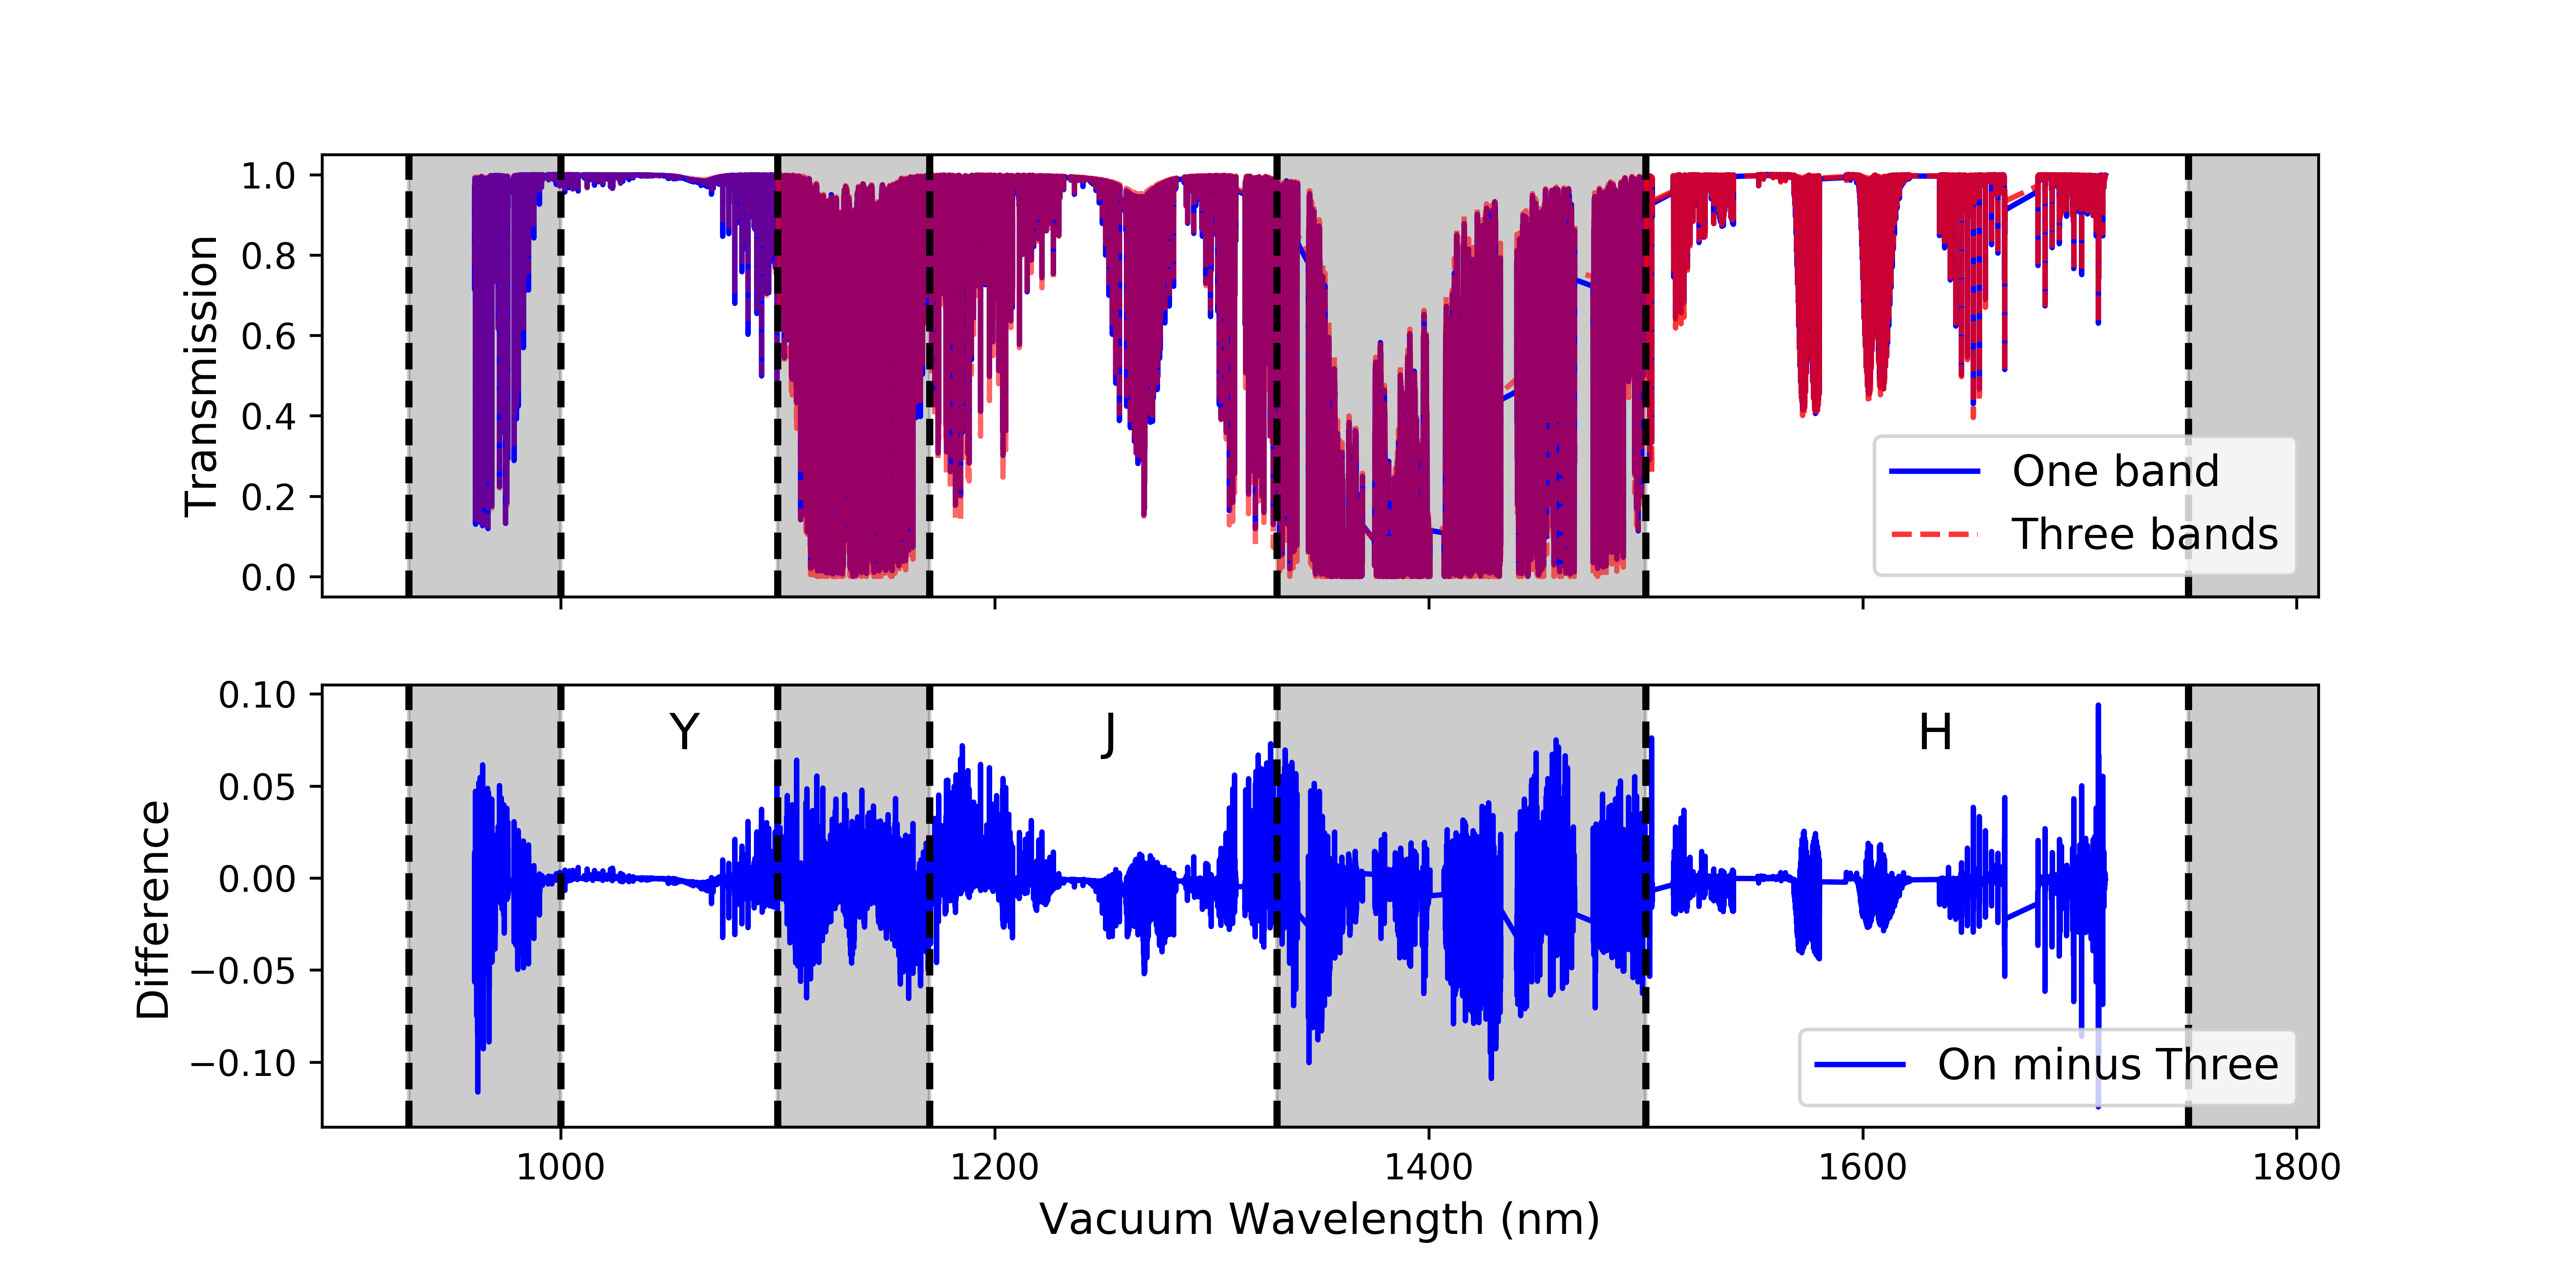
\includegraphics[width=0.9\linewidth]{figures/information-content/Carmenes/compare_telluric_corrections_shaded}
    \caption[]{Comparison of telluric models in pursuit of a better correction.
        Top: The two synthetic telluric spectra.
        The blue shows the result from Molecfit after treating the full spectrum as one, with a single spectral profile, while the shaded red telluric spectrum has been derived with three separate bands, fitted individually.
        Bottom: The difference in the telluric spectrum between the fit to the full spectrum, and the three individual fit.
        The regions of deep \ce{H2O} absorption lines which defined the \nir{} bands are shaded grey.
        The bounds of each band from \cref{tab:infrared_bands} are indicated with vertical black dashed lines.}
    \label{fig:compare_telluric_corrections}
\end{figure}


\begin{figure}
    \centering
    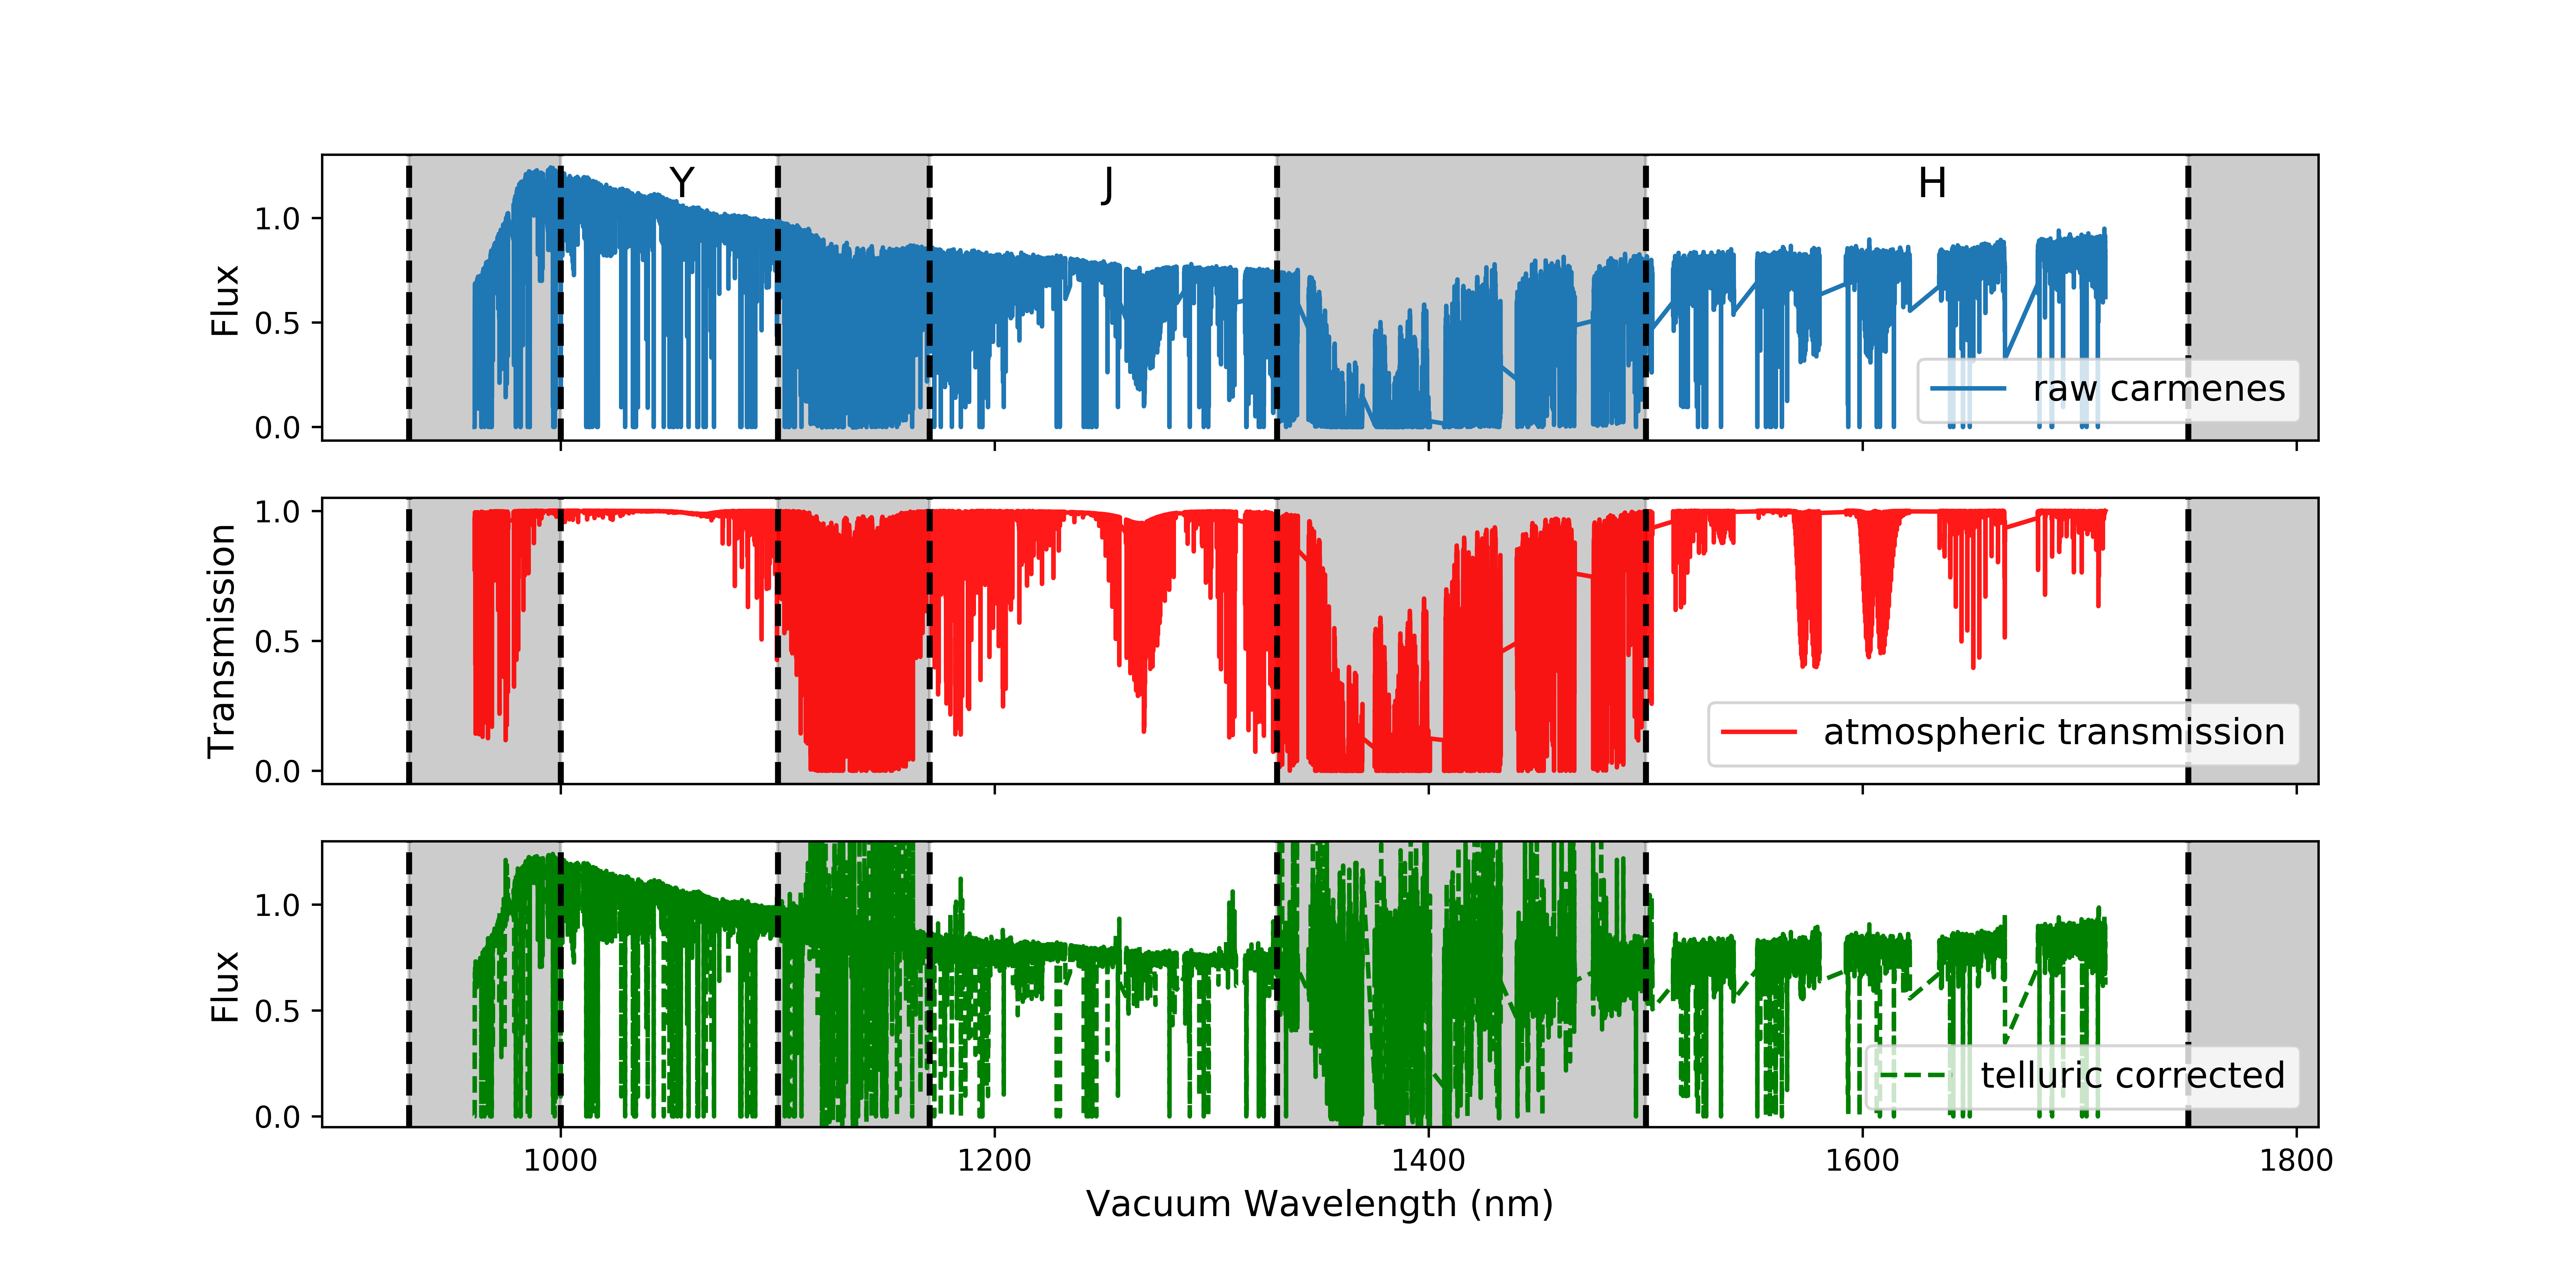
\includegraphics[width=0.9\linewidth]{figures/information-content/Carmenes/telluric_correct_carmenes}
    \caption[Telluic correction of the {CARMENES} \nir{} spectrum.]{Telluic correction of the {CARMENES} \nir{} spectrum.
    Top: Uncorrected spectrum of Barnard's Star between 960--1710\nm{} from {CARMENES}.
    Middle: The synthetic telluric transmission spectrum fitted with Molecfit.
    Bottom: Telluric corrected spectrum by division of the telluric spectrum.
    The regions of deep \ce{H2O} absorption lines which defined the \nir{} bands are shaded grey.
    The bounds of each band from \cref{tab:infrared_bands} are indicated with vertical black dashed lines.}
    \label{fig:carmenes_correction}
\end{figure}


\begin{figure}
    \centering
    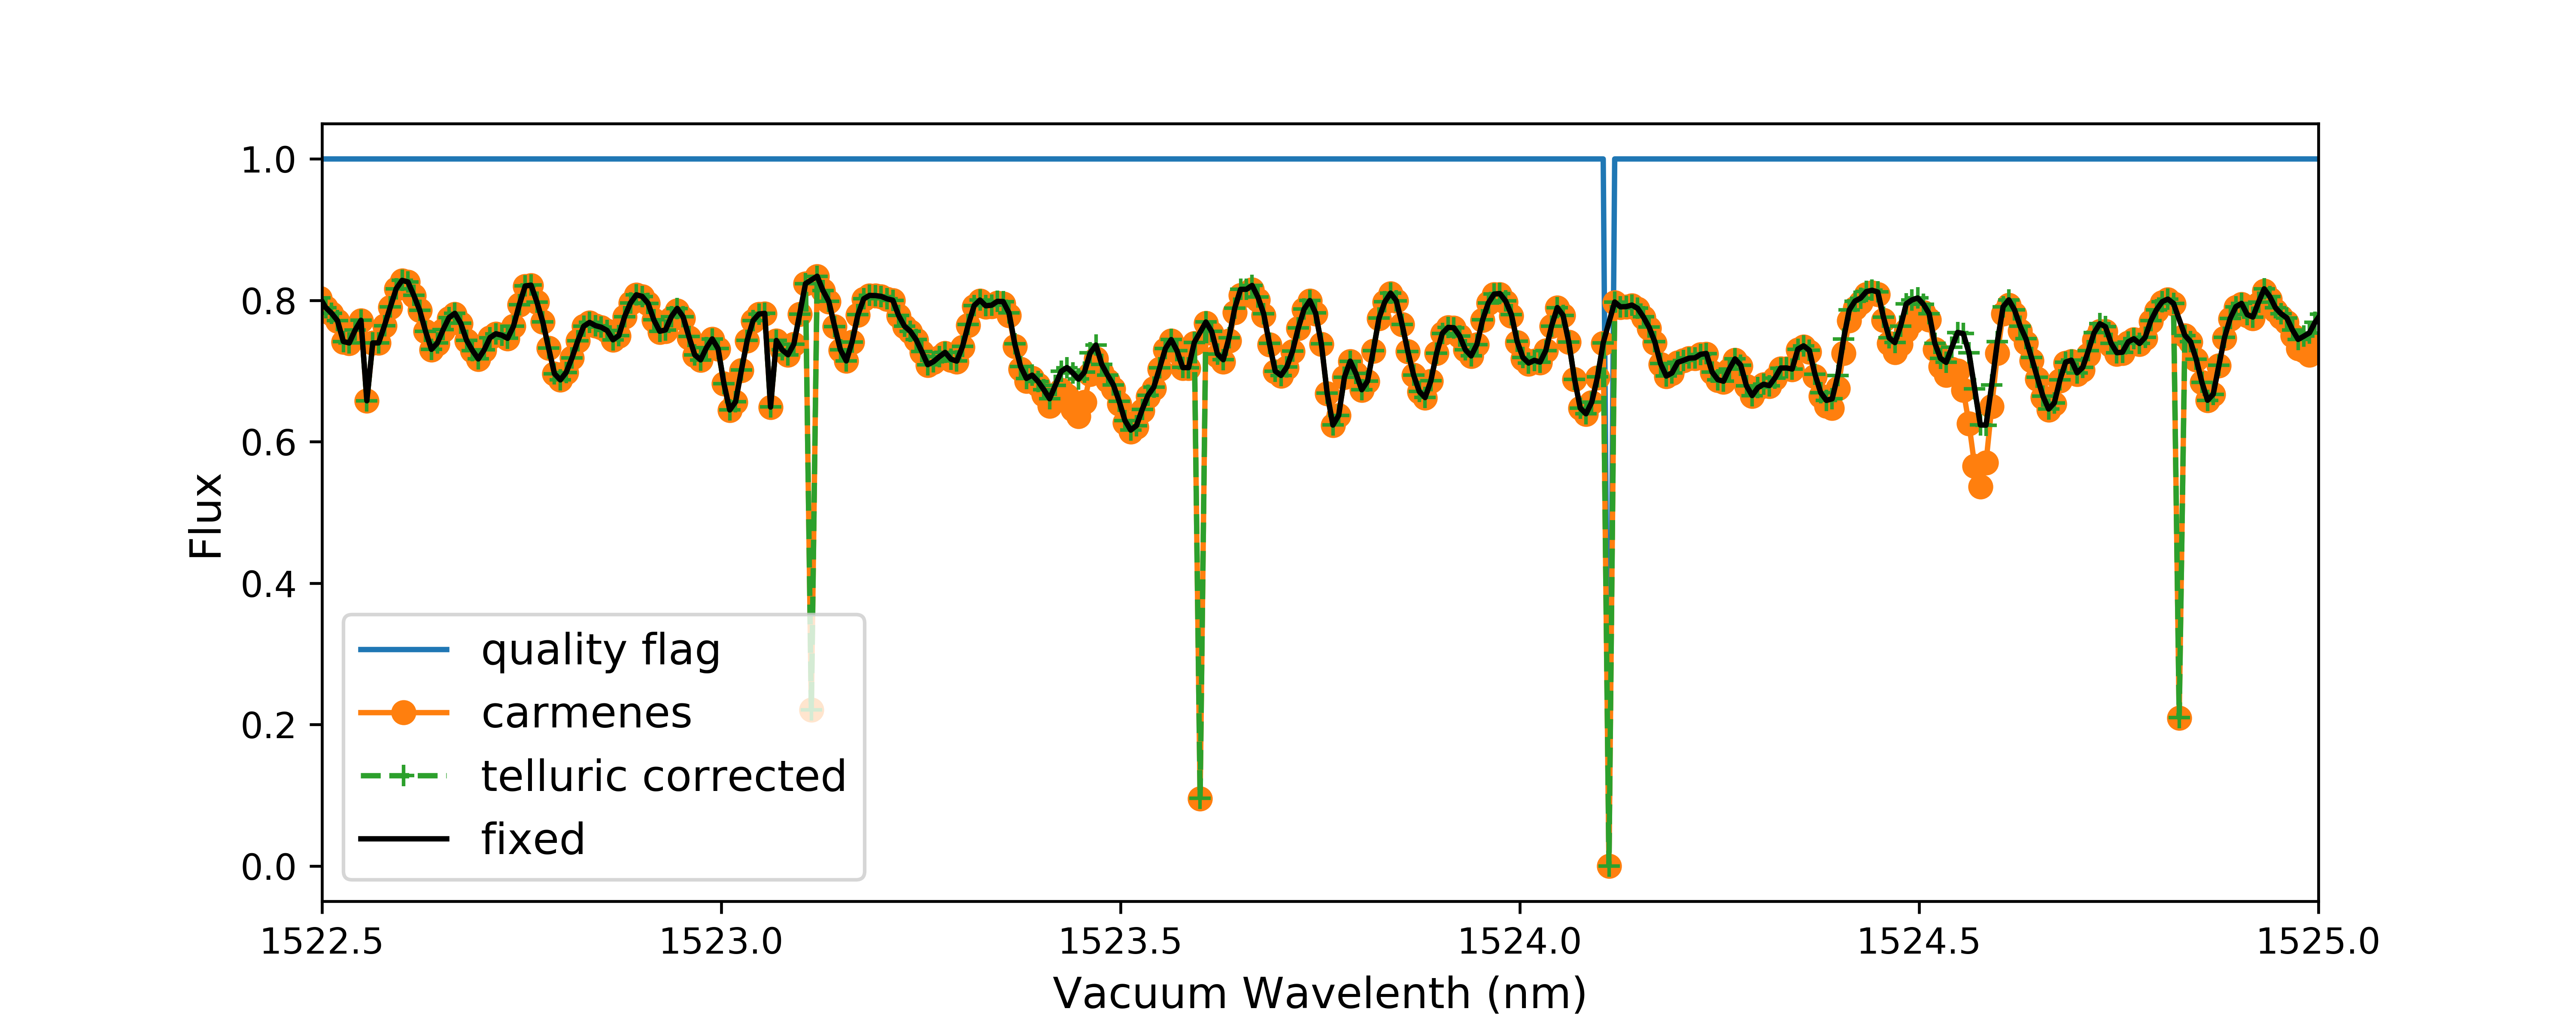
\includegraphics[width=0.9\linewidth]{figures/information-content/Carmenes/carmenes_spike_removal}
    \caption[]{Removal in bad pixels in CARMENES spectrum.}
    \label{fig:carmenes_spike_removal}
\end{figure}



The current implementation of the telluric correction has the spectrum broken into three chunks with the line profile of the lines fitted independently in each chunk.
Some regions have an improved telluric correction for while other regions the correction worsens.

\subsection{Barnard's star}
- Barnard's star (Artigau 2018 comparison)

Figure \citep{} shows the uncorrected {CARMENES} spectrum (xxx) along with the current telluric model (black) the bottom panel shows the corrected {CARMENES} spectrum after division.
The main \nir{} \ce{H2O} bands are also excluded outside the lines...


This work is work in progress.
{I can calculate the {RV} precision from models though.}




This work added an extra feature to \eniric{} in the ability to calculated spectra on a shorter wavelength scale such as 2\% widths as done in \citep{artigau_optical_2018}.


\subsection{Comparing models to {CARMENES}.}
Already somewhat done in Reiners.
(use all spectra).
They measured the precision obtained in the spectra.

Band by band like~\citet{figueira_radial_2016}?
Certain\% steps like Bouchy or Artigau


Can do Barnard's star in {CARMENES}.
\todo{finish this} compared to models in Artigau.

%% Old tables

%\DTLsetseparator{,}
%\DTLloadrawdb{targets}{data/carmenes_selection.csv}%
%
%\begin{table*}[h]
%    \centering
%    \caption[Selection of targets from the {CARMENES} library.]{Selection of targets from the {CARMENES} library spanning the {M-dwarf} spectral range.}
%    \begin{tabular}{l l l r c c c c}%
%        \toprule
%        Karmn & Name & SpT &  \({\snr{}}_{\textrm{NIR}}\)  & Temp (K)  & \Logg{} & \feh{} & v\(\sin{i}\) (\kmps{})\\
%        \midrule
%        \DTLforeach*{targets}{\id=Karmn,\name=Name,\sptype=SpT,\SNR=NIR-SNR,\TEFF=Teff, \LOGG=logg,\metal=FeH, \rot=ROT-Vsini}{
%            \DTLiffirstrow{}{\\}\id{} & \name{}  & \sptype{} & \SNR{} & \TEFF{} & \LOGG{} & \metal{} & \rot{}
%        }
%        \\
%        \bottomrule
%    \end{tabular}
%    \label{tab:targets}
%\end{table*}

%%!TEX root = ../thesis.tex

\begin{table}[h]
    \caption[CARMENES targets for RV precision analysis.]{csv2tex table}
    \begin{tabular}{lllrrrrr}
        \toprule
        Karmn &            Name &   SpT &  \nir{}-\snr &    \Teff{} & \Logg{} & \feh{} &  ROT-\Vsini{} \\
        \midrule
        J20533+621 &      BD+61 2068 &  M0.5 &      257 &  3\,772.0 &     - & -0.01 &       2.66 \\
        J04290+219 &       BD+21 652 &  M0.5 &      212 &  4\,037.0 &  3.99 & -0.21 &       1.11 \\
        J07274+052 &   Luyten's Star &  M3.5 &      254 &  3\,467.0 &     - & -0.11 &          - \\
        J17578+046 &  Barnard's Star &  M3.5 &      236 &  3\,247.0 &     - & -0.32 &          - \\
        J11055+435 &          WX UMa &  M5.5 &      140 &  3\,304.0 &     - &     - &          - \\
        J10564+070 &          CN Leo &  M6.0 &      133 &  2\,960.0 &     - &     - &          - \\
        J18356+329 &  LSR J1835+3259 &  M8.5 &       50 &  2\,578.0 &     - & -0.40 &      37.60 \\
        J04198+425 &  LSR J0419+4233 &  M8.5 &       42 &       - &     - &  0.22 &          - \\
    \bottomrule
    \end{tabular}\label{tab:carmenes_selection}
\end{table}

%\begin{table}
\label{}
\caption{csv2tex table transposed}
\begin{tabular}{lllllllll}
\toprule
{} &           0 &           1 &              2 &               3 &           4 &           5 &               6 &               7 \\
\midrule
Karmn     &  J20533+621 &  J04290+219 &     J07274+052 &      J17578+046 &  J11055+435 &  J10564+070 &      J18356+329 &      J04198+425 \\
Name      &  BD+61 2068 &   BD+21 652 &  Luyten's Star &  Barnard's Star &      WX UMa &      CN Leo &  LSR J1835+3259 &  LSR J0419+4233 \\
SpT       &        M0.5 &        M0.5 &           M3.5 &            M3.5 &        M5.5 &        M6.0 &            M8.5 &            M8.5 \\
NIR-SNR   &         257 &         212 &            254 &             236 &         140 &         133 &              50 &              42 \\
Teff      &        3772 &        4037 &           3467 &            3247 &        3304 &        2960 &            2578 &               - \\
logg      &           - &        3.99 &              - &               - &           - &           - &               - &               - \\
FeH       &       -0.01 &       -0.21 &          -0.11 &           -0.32 &           - &           - &            -0.4 &            0.22 \\
ROT-Vsini &        2.66 &        1.11 &              - &               - &           - &           - &            37.6 &               - \\
\bottomrule
\end{tabular}
\end{table}

